\documentclass[11pt]{article}

\usepackage[margin=1in]{geometry}
\usepackage{natbib}
\usepackage{booktabs}
\usepackage{amsmath}
\usepackage{amssymb}
\usepackage{hyperref}
\usepackage{url}
\usepackage{xspace}
\usepackage{graphicx}

\newcommand{\method}{TurboQuant-MSE\xspace}
\newcommand{\erel}{E_{\mathrm{rel}}}

\title{Compressing the Latent Communication Channel of a\\
Recursive Multi-Agent System: An Empirical Study}
\author{[author]\\\texttt{[email]}}
\date{2026}

\begin{document}
\maketitle

\begin{abstract}
We ask whether the latent vectors that agents in a recursive multi-agent system
exchange can be compressed without harming downstream accuracy. The question is
not obvious: unlike the KV cache --- the usual target of activation quantization,
where each entry is averaged over many attention queries --- a message in this
latent channel is consumed once, without averaging, through a bottleneck, and
repeatedly along the recursion. We inject the MSE-optimal core of TurboQuant
\citep{turboquant2026} --- a data-oblivious Haar rotation followed by
per-coordinate Lloyd--Max scalar quantization, without the QJL inner-product
residual --- into every latent link of RecursiveMAS Sequential-Light
\citep{recursivemas2026}, and measure its effect on math500 at three granularities:
per-link reconstruction error, end-to-end accuracy, and the per-step output
distribution. The per-link error tracks the quantizer's reported distortion rate
($\erel\approx0.009$ at 4 bits), and under sampled decoding we detect no accuracy
change from $4\times$ to $16\times$ compression at $n{=}250$. Our most informative
result is a qualifier: under deterministic greedy decoding the compressed channel
is \emph{answer-preserving but not trajectory-preserving} --- the 4-bit channel
changes the generated reasoning text in 88\% of problems while preserving the final
answer, and a strict $\pm2$-point paired equivalence test is inconclusive
($\Delta=-2.0$ pp, 95\% CI $[-6.4,+2.4]$). This is a focused study of one released
system on one benchmark under fake-quantization; we report what we measured and
bound what we did not.
\end{abstract}

\section{Introduction}

Multi-agent systems built from heterogeneous language models increasingly
communicate in latent space rather than in text: one agent projects its
last-layer hidden state and hands it to another. RecursiveMAS
\citep{recursivemas2026} formalizes this with a lightweight recursive link that
transmits an agent's hidden state across agents of different hidden sizes. As such
systems move toward distributed deployment, the bandwidth of this latent channel
becomes a practical cost, which raises a concrete question: how compressible is it?

Activation quantization is well studied for the KV cache, which is unusually
tolerant. Each cached key/value is averaged over many attention queries, softmax
attenuates per-token noise, and the outliers are structured. The latent
communication channel has none of these properties. It is a one-shot message --- the
receiving agent consumes it once, with no averaging. It is an information-dense
bottleneck (a two-layer residual MLP with LayerNorms). And it is traversed
repeatedly along the recursion, so per-call errors could in principle compound. A
priori it is unclear whether this channel behaves like the compressible KV cache or
like a fragile final-layer logit.

We answer the question empirically. We take TurboQuant's MSE-optimal quantizer
unchanged from \citet{turboquant2026} --- a data-oblivious Haar rotation, which
concentrates the per-coordinate marginal, followed by an optimal scalar quantizer
--- and inject it into every link of RecursiveMAS Sequential-Light. We then measure
math500 accuracy and output fidelity, and we contrast sampled with deterministic
greedy decoding so that we can attribute effects cleanly.

\paragraph{Contributions.}
\begin{itemize}
  \item We frame the latent communication channel of a recursive multi-agent system
  as a compression target distinct from the KV cache, and give an
  instrumentation-only methodology: the model and the quantizer are untouched.
  \item Under sampled decoding, we detect no math500 accuracy change from $4\times$
  to $16\times$ compression at $n{=}250$ (two-proportion $z$-tests, all $p>0.4$).
  \item Under deterministic greedy decoding, the compressed channel is
  \emph{answer-preserving but not trajectory-preserving}: the 4-bit channel changes
  the generated text in 88\% of problems, yet the paired accuracy difference is
  small and a $\pm2$-point equivalence test is inconclusive
  ($\Delta=-2.0$ pp, CI $[-6.4,+2.4]$). A REF-vs-REF control attributes the change
  to the quantizer rather than to nondeterminism.
  \item We document two reproducibility hazards: bfloat16 silently collapses this
  recursive pipeline on pre-Ampere GPUs, and an injected quantizer's internal dtype
  must match the pipeline's.
\end{itemize}

This is a study, not a new method: the quantizer and the system are both taken
unchanged from prior work \citep{turboquant2026,recursivemas2026}. We evaluate the
MSE core of TurboQuant, not the complete algorithm with its QJL residual
(Section~\ref{sec:method}).

\section{Background and related work}

\paragraph{Activation and KV-cache quantization.} A substantial literature
compresses LLM key/value caches to low bit-rates with little quality loss,
exploiting the statistical redundancy and averaging inherent to attention. Our
target differs structurally --- a one-shot, bottlenecked, repeatedly-traversed
latent message rather than an averaged cache entry --- so tolerance does not
transfer by assumption, which is what motivates a direct measurement.

\paragraph{Data-oblivious vector quantization.} TurboQuant
\citep{turboquant2026} attains near-optimal distortion with a random rotation
followed by an optimal per-coordinate scalar quantizer, and requires no calibration
data. It has two components: an MSE-optimal quantizer, and a QJL inner-product
residual for inner-product-preserving tasks. We use only the MSE-optimal core
(Section~\ref{sec:method}); the data-oblivious property is what makes a drop-in
deployment plausible in the first place.

\paragraph{Recursive multi-agent systems.} RecursiveMAS \citep{recursivemas2026}
connects heterogeneous agents through a recursive latent link. We treat its
released Sequential-Light constellation as a fixed system and study only the
compressibility of its latent communication channel; we modify neither the agents
nor the link weights.

\section{Method}
\label{sec:method}

\paragraph{The quantizer.} We instantiate the MSE-oriented core of TurboQuant,
which we refer to as \method{}. Given a channel vector $x\in\mathbb{R}^d$, \method{}
normalizes $x$ onto the unit sphere, applies a fixed Haar-random rotation $R$
(computed once and stored as a buffer), quantizes each rotated coordinate with a
$2^b$-level Lloyd--Max codebook precomputed for the concentrated marginal, then
inverts the rotation and rescales. The quantizer is data-oblivious, carries no
per-tensor scale or group size, and works at any $d$. We do \emph{not} include
TurboQuant's QJL inner-product residual, which targets inner-product preservation;
our intervention replaces dense latent vectors at the communication boundary, so it
targets direct reconstruction fidelity. This narrows the claim to a \method{}
instantiation rather than the complete TurboQuant algorithm, and it sharpens the
empirical point: the MSE core alone suffices for the final-answer robustness we
measure. We verified our implementation against the reference numerically (codebook
and rotation match to $10^{-4}$, end-to-end reconstruction to $5\times10^{-4}$) and
against the reported distortion rate (Section~\ref{sec:distortion}).

\paragraph{Insertion point.} RecursiveMAS routes each latent transfer through an
adapter that ends in a LayerNorm. We wrap each adapter's forward pass so its
post-LayerNorm output passes through \method{} before being returned. Quantization
runs in fp32, and the result is cast back to the pipeline dtype. The wrapper is
reversible and records per-call distortion; the model and quantizer code are never
edited.

\paragraph{Measurement.} We evaluate at three granularities. (i) \emph{Per-link
distortion}: the relative squared reconstruction error
$\erel=\lVert x-\hat x\rVert_2^2/\lVert x\rVert_2^2$ and the cosine similarity, at
every adapter call. (ii) \emph{End-to-end accuracy} on math500. (iii) \emph{Per-step
output fidelity}: for a paired unquantized (REF) and 4-bit (INT4) run under greedy
decoding with a shared seed, we capture the top-$K{=}512$ next-token logits at each
decode position and compute the KL divergence, the Jensen--Shannon divergence, and a
probability-space MSE between the two distributions. Because the two greedy
trajectories can diverge --- after which a positional comparison is meaningless ---
we report (iii) only over the matched prefix (the positions up to and including the
first token at which the two runs choose different tokens), and we report the
divergence rate separately. We sweep the channel-traversal count
$T=\texttt{num\_recursive\_rounds}\in\{1,2,3,4\}$, and we compare accuracy with a
paired bootstrap and a two one-sided test (TOST) for equivalence at a
\emph{pre-specified} margin of $\varepsilon{=}2$ percentage points (pp).

\paragraph{A note on the equivalence verdict.} TOST certifies equivalence only when
both one-sided tests reject. When neither rejects, equivalence is simply \emph{not
established}; we report this as ``inconclusive'' and never as evidence that the two
conditions differ.

\section{Experiments}

All runs use math500, seed 42, and fp32. Compute is a single A100-40GB (Modal) for
the paired greedy analysis and a single T4 (Kaggle, fp32) for the sampled ladder.
Two decoding regimes carry different baselines, and we never compare across them
(Table~\ref{tab:baselines}): the sampled ladder uses the released sampling settings
with \emph{unpaired} runs, while the fidelity and equivalence analyses use greedy
decoding with \emph{paired} REF/INT4 runs on identical inputs. A separate $n{=}50$
exploration baseline of $\sim$84\% reflects an easier subset and is not comparable
to either powered baseline.

\begin{table}[t]
\centering
\caption{Baselines are experiment-specific; we do not compare across decoding
regimes. Sampled = unpaired runs under the released sampling settings; greedy =
paired REF/INT4 on identical inputs.}
\label{tab:baselines}
\begin{tabular}{llccl}
\toprule
experiment & decoding & $n$ & baseline & treatment \\
\midrule
sampled ladder (T4 fp32) & sampled & 250 & 75.2\% & 8/4/2-bit: 78.4/76.8/75.2\% \\
greedy paired (A100 fp32, $T{=}3$) & greedy & 250 & REF 76.8\% & INT4 74.8\% \\
REF-vs-REF control & greedy & 250 & 76.8\% & 76.8\% ($\Delta0$) \\
depth sweep & greedy & 50 & per-$T$ & INT4 \\
\bottomrule
\end{tabular}
\end{table}

\subsection{Per-link distortion tracks the reported rate}
\label{sec:distortion}

On the real Solver adapter output (dimension $1536$), the relative squared error of
\method{} follows the same rate curve as a synthetic Gaussian baseline and the
values reported by \citet{turboquant2026}; agreement is close at the bit-rates used
downstream (Table~\ref{tab:distortion}), tightest at 8 and 4 bits and looser at
3 bits. The latent channel is therefore compressible by TurboQuant, and the
data-oblivious property holds on a real channel without calibration.

\begin{table}[t]
\centering
\caption{Per-link relative squared reconstruction error
$\erel=\lVert x-\hat x\rVert_2^2/\lVert x\rVert_2^2$ of \method{} on the real
adapter output, versus synthetic data and the reported TurboQuant distortion rate
(lower is better).}
\label{tab:distortion}
\begin{tabular}{lccc}
\toprule
bits & synthetic ($d{=}2048$) & real adapter ($d{=}1536$) & reported \citep{turboquant2026} \\
\midrule
8 & 0.0001 & 0.0001 & ($\approx$lossless) \\
4 & 0.0095 & 0.0093 & 0.009 \\
3 & 0.0345 & 0.0339 & 0.030 \\
2 & 0.1175 & 0.1159 & 0.117 \\
\bottomrule
\end{tabular}
\end{table}

\subsection{Sampled decoding: no detected accuracy change at $4\times$--$16\times$}
\label{sec:accuracy}

We inject \method{} at every link and evaluate math500 at $n{=}250$ under sampled
decoding. We do not detect an accuracy change from the unquantized baseline at any
bit-rate from 8 down to 2 (Table~\ref{tab:ladder} and Figure~\ref{fig:ladder};
two-proportion $z$-tests, all $p>0.4$; the 95\% Wald intervals for every delta
straddle zero). At 2 bits per coordinate --- a $16\times$ reduction, near the
information-theoretic floor --- the quantized system reaches the same accuracy count
as baseline ($188/250$). This is consistent with no degradation at the resolution of
this experiment; it is not a proof of equality (Section~\ref{sec:greedy} probes the
channel more finely).

\begin{table}[t]
\centering
\caption{Math500 accuracy at $n{=}250$ under sampled decoding (T4, fp32). We detect
no difference from baseline at any bit-rate (two-proportion $z$-test, all $p>0.4$);
95\% intervals are Wald two-proportion-difference intervals.}
\label{tab:ladder}
\begin{tabular}{lcccc}
\toprule
bits/coord & compression & accuracy & $\Delta$ baseline (95\% CI) & $p$ \\
\midrule
-- (baseline) & $1\times$ & 75.2\% & -- & -- \\
8 & $4\times$ & 78.4\% & $+3.2$ $[-4.2,+10.6]$ & $>0.4$ \\
4 & $8\times$ & 76.8\% & $+1.6$ $[-5.9,+9.1]$ & $>0.5$ \\
2 & $16\times$ & 75.2\% & $0.0$ $[-7.6,+7.6]$ & $1.0$ \\
\bottomrule
\end{tabular}
\end{table}

\begin{figure}[t]
\centering

\includegraphics[width=0.6\linewidth]{figures/bit_rate_ladder_n250.png}
\caption{Math500 accuracy versus \method{} bit-rate at $n{=}250$ under sampled
decoding. The curve is flat from the unquantized baseline through $16\times$
compression; every bit-rate lies within sampling noise of the baseline. Under greedy
decoding a stricter paired equivalence test is inconclusive
(Section~\ref{sec:greedy}).}
\label{fig:ladder}
\end{figure}

\paragraph{What this buys, information-theoretically.} For the powered $T{=}3$
configuration, the all-link run quantizes $1{,}152$ latent token-vectors per math500
problem ($288{,}000$ over $250$ problems). With a representative channel dimension
$d\approx2048$ (agent hidden sizes span $1536$--$2048$), the per-problem latent
traffic is
\[
\mathrm{traffic} \;=\; N_{\text{vectors}}\times d \times \tfrac{b}{8}
\;\approx\; 1{,}152 \times 2048 \times \tfrac{b}{8}\ \text{bytes},
\]
i.e.\ $\approx 9.0$ MiB at fp32 ($b{=}32$), $\approx 1.1$ MiB at 4 bits, and
$\approx 0.56$ MiB at 2 bits. These are information-theoretic, packed-integer
figures; we measure fake-quantization fidelity, not wall-clock bandwidth or latency
(Section~\ref{sec:limits}).

\subsection{Greedy decoding: answer-preserving, not trajectory-preserving}
\label{sec:greedy}

Accuracy is a one-bit-per-problem metric. To probe the channel more finely we run a
paired REF-vs-INT4 comparison under deterministic greedy decoding at $n{=}250$,
$T{=}3$. The 4-bit run scores $74.8\%$ against the unquantized $76.8\%$: a paired
difference of $-2.0$ pp with a 95\% bootstrap interval of $[-6.4,+2.4]$. At the
pre-specified $\varepsilon{=}2$-pp margin the equivalence test is inconclusive ---
the estimate sits on the margin and the interval reaches $-6.4$ pp, so we establish
neither equivalence nor a difference (Table~\ref{tab:tost}). The sampled ladder of
Section~\ref{sec:accuracy} and this greedy estimate are not directly comparable
(different decoding, different unpaired vs paired runs); both effects are small, and
we summarize across regimes as: the 4-bit accuracy effect is at most a few points
and not robustly distinguishable from zero.

\begin{table}[t]
\centering
\caption{Paired accuracy and TOST equivalence ($\varepsilon{=}2$pp) under greedy
decoding at $T{=}3$, $n{=}250$. ``Inconclusive'' means equivalence was not
established, not that the conditions differ.}
\label{tab:tost}
\begin{tabular}{lccc}
\toprule
comparison & $\Delta$acc (95\% CI) & TOST verdict & $n$ \\
\midrule
INT4 vs REF & $-2.0$ $[-6.4, +2.4]$ & inconclusive & 250 \\
REF vs REF (control) & $0.0$ $[0.0, 0.0]$ & --- & 250 \\
\bottomrule
\end{tabular}
\end{table}

\paragraph{The effect is the quantizer, not nondeterminism.} We run the unquantized
configuration twice. The two runs are bit-identical: zero problems differ, zero
trajectory divergence, zero per-step KL (Table~\ref{tab:tost}, control row). The
pipeline is therefore deterministic across containers, and any REF-vs-INT4
difference is attributable to the quantizer rather than to run-to-run noise.

\paragraph{The quantizer changes the trajectory but not the answer.} Although the
accuracy effect is small, the 4-bit channel changes the generated tokens
substantially. On the clean $n{=}250$ run, the greedy trajectory eventually selects
a different token from the unquantized run in $88\%$ of problems (divergence rate
$0.88$), after a mean matched prefix of $\approx80$ tokens (against a control
divergence rate of zero). Over those matched prefixes the output distributions are
measurably but modestly shifted, not zero: matched-prefix KL $0.325$ nats
(95\% CI $[0.162,0.512]$) and Jensen--Shannon $0.032$ ($[0.018,0.047]$), with a
per-call channel cosine of $0.9954$ (relative L2 $\approx0.096$, consistent with the
4-bit rate). The 4-bit channel thus changes the \emph{reasoning text} in most
problems while the \emph{final answer} survives: the compressed channel is
answer-preserving, not trajectory-preserving.

\subsection{Depth and link localization}
\label{sec:depth}

\paragraph{Depth.} Across $T\in\{1,2,3,4\}$ the system's accuracy does not collapse,
so the catastrophic per-call-error accumulation one might fear a priori
($\sim\varepsilon\cdot N$ over $N$ channel calls) does not occur. We avoid a stronger
depth claim. The per-call channel cosine is $0.9954$ at every $T$
(Figure~\ref{fig:cosine}), but this is depth-independent \emph{by construction} ---
the quantizer is data-oblivious, so its per-call distortion depends only on bit-rate
and dimension --- and is a consistency check, not a depth result. Our finer per-step
KL estimator is too unstable to resolve a depth trend: at the same $T{=}3$ it reads
$0.03$ at $n{=}50$ and $0.33$ at $n{=}250$, and it averages over run-dependent
positions.

\begin{figure}[t]
\centering
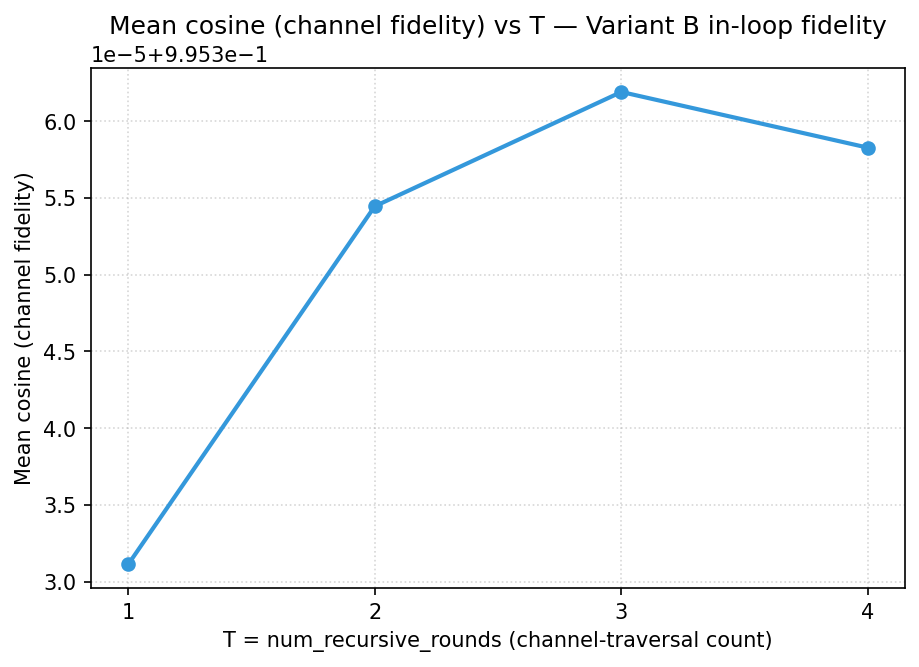
\includegraphics[width=0.6\linewidth]{figures/fidelity_cosine_vs_T.png}
\caption{Per-call channel cosine (4-bit round-trip) versus recursion depth $T$. The
cosine is $\approx0.9954$ at every $T$ --- a consistency check, since the
data-oblivious quantizer's per-call distortion is depth-independent by construction,
not a depth result.}
\label{fig:cosine}
\end{figure}

\paragraph{Localization.} The channel splits into same-model inner links
(intra-agent recursion, $\sim$12{,}544 calls) and cross-model outer links (the
genuinely inter-agent transfers, $\sim$256 calls). We quantize each in isolation to
ask which carries the small accuracy cost (Table~\ref{tab:localize}). The question is
not resolved at $n{=}250$: the three paired deltas ($-0.8$, $-1.2$, $-2.0$ pp) all
have 95\% intervals that straddle zero and overlap heavily, so we cannot attribute
the cost to either link type. The divergence-rate metric does not help either --- it
is a saturating binary near $0.88$ for the all-link run and cannot separate
conditions. Both link types plausibly contribute; resolving their relative
contribution would require a position-aligned (teacher-forced) per-step measurement
that we did not run.

\begin{table}[t]
\centering
\caption{Selective quantization at $T{=}3$, $n{=}250$, greedy (clean retry). The
paired accuracy deltas do not resolve whether inner or outer links carry the small
cost: all 95\% intervals straddle zero and overlap.}
\label{tab:localize}
\begin{tabular}{lccc}
\toprule
quantized & \#calls & accuracy & $\Delta$acc vs REF (95\% CI) \\
\midrule
REF (none) & 0 & 76.8\% & -- \\
inner only & 12{,}544 & 76.0\% & $-0.8$ $[-5.2, +3.6]$ \\
outer only & 256 & 75.6\% & $-1.2$ $[-5.6, +3.2]$ \\
both & 12{,}800 & 74.8\% & $-2.0$ $[-6.4, +2.4]$ \\
\bottomrule
\end{tabular}
\end{table}

\subsection{Reproducibility hazards}
\label{sec:hazards}

\paragraph{bfloat16 on pre-Ampere GPUs.} The released checkpoints specify bfloat16,
and the default loader uses it. On GPUs without native bf16 support (compute
capability below 8.0: P100, V100, T4) the recursive rollouts silently collapse
math500 accuracy to $\sim$30--35\%; forcing fp32 restores it to $\sim$84\% on the
same hardware. The collapse is a deep-recursion effect; single-forward use is
unaffected.

\paragraph{Dtype mismatch.} Placing the fp32-internal quantizer inside a bf16
pipeline introduces a cast between bf16 and fp32 at each of $\sim$48 calls; the casts
accumulate ${\sim}10^{-3}$ error per call and manufacture a spurious $-19$-point
accuracy drop. A dtype-coherent (fp32) pipeline removes it. An injected quantizer's
internal dtype must match the pipeline it is measured in.

\section{Discussion}
\label{sec:discussion}

\paragraph{What the result means.} The compressed channel is answer-preserving but
not trajectory-preserving. Aggressive data-oblivious quantization of the latent
messages does not keep the generated reasoning identical --- it changes the
trajectory in most problems --- yet the final answer survives. The robustness we
measure is therefore a property of the \emph{task and system}, whose redundancy lets
a perturbed latent thought still land on the right answer, rather than evidence of a
noise-free channel.

\paragraph{Does the error propagate?} Yes, and we do not claim otherwise. The 4-bit
perturbation propagates far enough to change the greedy trajectory in 88\% of
problems and to shift the matched-prefix output distribution (KL $\approx0.33$ nats).
What we observe is that this propagation does not \emph{amplify} into an accuracy
collapse as recursion depth grows to $T{=}4$, and that per-call input distortion is
bounded and depth-independent by construction. We cannot certify that the propagated
distortion is uniformly small: our per-step KL estimate is unstable across sample
sizes ($0.03$ at $n{=}50$ vs $0.33$ at $n{=}250$), and we did not run a
teacher-forced per-step measurement.

\paragraph{Why it matters.} Latent communication is proposed as the efficient
alternative to text-based agent messaging. If that latent channel is \emph{also}
highly compressible at no detected accuracy cost, the efficiency argument compounds.
This study gives narrowly-scoped evidence that a real recursive multi-agent latent
channel tolerates $4\times$--$16\times$ data-oblivious compression, and it
characterizes the failure mode --- trajectory drift under preserved answers --- that
a deployment would need to monitor. It does not establish a deployable bandwidth
saving, generality beyond this system, or unconditional losslessness.

\section{Limitations}
\label{sec:limits}

We measure \emph{fake}-quantization fidelity: the dequantized vector is exactly what
a packed low-bit transport would deliver, so the accuracy and distribution numbers
are faithful, but we report no measured wall-clock bandwidth, latency, or memory
saving; the traffic figures in Section~\ref{sec:accuracy} are information-theoretic.
We evaluate only the MSE core of TurboQuant; the QJL inner-product residual is an
untested future ablation, especially at lower bit-rates or inner-product-dominated
objectives. The accuracy equivalence analysis is at $n{=}250$ for $T{=}3$; the depth
sweep is at $n{=}50$, which underpowers a per-$T$ equivalence test. Our per-step KL
is a matched-prefix proxy rather than a position-aligned (teacher-forced)
measurement, and is too unstable to support a depth or localization conclusion. All
results use a single seed, a single benchmark (math500), a single subset ordering,
and a single released constellation (Sequential-Light); we make no claim of
generality. Finally, the quantizer and the system are both taken unchanged from prior
work; the contribution is the measurement, not a method.

\section{Conclusion}

The latent communication channel of a recursive multi-agent system --- one-shot,
bottlenecked, and repeatedly traversed --- is highly compressible by the MSE core of
a data-oblivious quantizer: under sampled decoding we detect no math500 accuracy
change from $4\times$ to $16\times$ at $n{=}250$, and accuracy does not collapse as
recursion depth grows. The honest qualifier is that under deterministic greedy
decoding the compressed channel is answer-preserving but not trajectory-preserving:
it changes the generated reasoning text in most problems and yields a small,
non-significant accuracy difference whose equivalence we cannot certify. The main
practical obstacle we met was not the quantizer but dtype handling, which we
document. Code, the reproducibility workflow, and post-hoc analysis scripts for every
experiment accompany this write-up.

\bibliographystyle{plainnat}
\bibliography{references}

\end{document}
